\section{Prezentacja wyników pracy - 10.05.2023r}
    Do dnia 10.05.2023r. dokonano następujących postępów:
        \begin{itemize}
            \item zaimplementowano odczyt danych z portu szeregowego, poprzez uruchomienie go w osobnym wątku. 
                Obiekt będący kontenerem na dane przekazywany jest przez wskaźnik do obiektu \textit{main\_window}, dzięki
                czemu dane są dostępne dla pozostałych komponentów aplikacji.
            \item zaprojektowano interfejs widoku ,,Temperatura'' (Rysunek \ref{fig: temp 10 05}),
            \item zaprojektowano interfejs okienka służącego ustawianiu wartości alarmów (Rysunek \ref{fig: alarms window 10 05}),
            \item połączono sloty odpowiedzialne za aktualizacje właściwych im danych dotyczących elementów interfejsu, takich jak:
                \begin{itemize}
                    \item graficzna i tekstowa  prezentacja wypełnienia silosu (widok ,,Wszystkie parametry''),
                    \item graficzna i tekstowa prezentacja temperatury (widoki ,,Wszystkie parametry'' i ,,Temperatura''),
                    \item Prezentacja informacji o alarmach  (widoki ,,Wszystkie parametry'' i ,,Temperatura'') (Rysunek \ref{fig: all param 10 05},\ref{fig: all param_2 10 05}),
                \end{itemize}
            \item przebudowano strukturę aplikacji, odciążono obiekt \textit{main\_window}, w którym znajdowały się 
                wszystkie sloty wykorzystywane przez aplikację. Utworzono klasy ,,backendowe'' w których usystematyzowano
                kod dotyczący  slotów.
        \end{itemize}

        \subsection{Aplikacja}
            Poniżej znajdują się zrzuty ekranu prezentujące wypracowany interface.
            \begin{figure}[H]
                \centering
                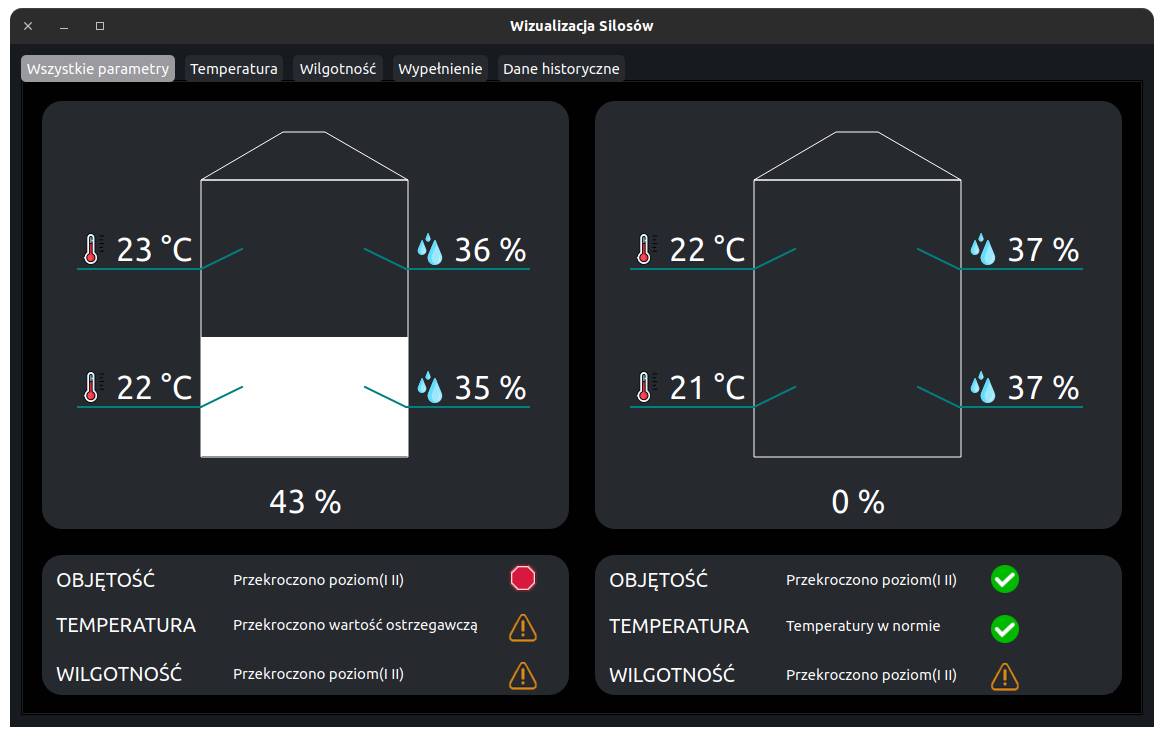
\includegraphics[width = \textwidth]{obrazy/all_param10_05_23.png}
                \caption{Wygląd zakładki wszystkie parametry}
                \label{fig: all param 10 05}
            \end{figure}

            \begin{figure}[H]
                \centering
                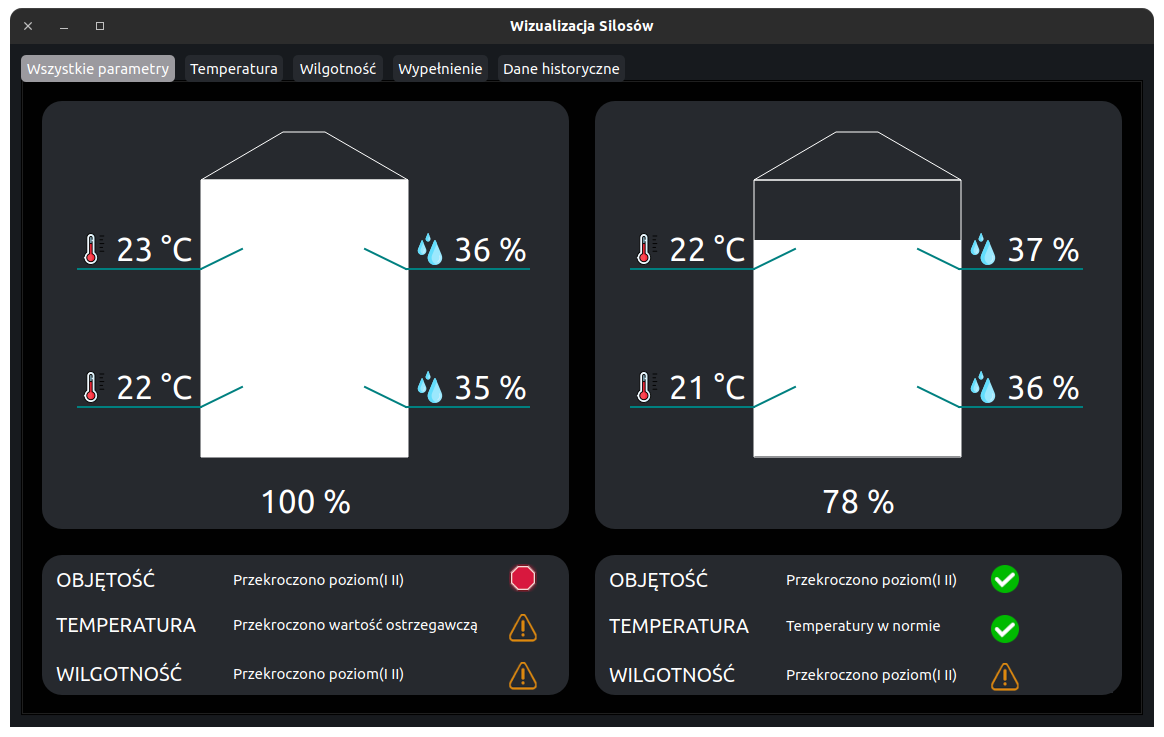
\includegraphics[width = \textwidth]{obrazy/all_param_10_05_2.png}
                \caption{Wygląd zakładki wszystkie parametry}
                \label{fig: all param_2 10 05}
            \end{figure}

            \begin{figure}[H]
                \centering
                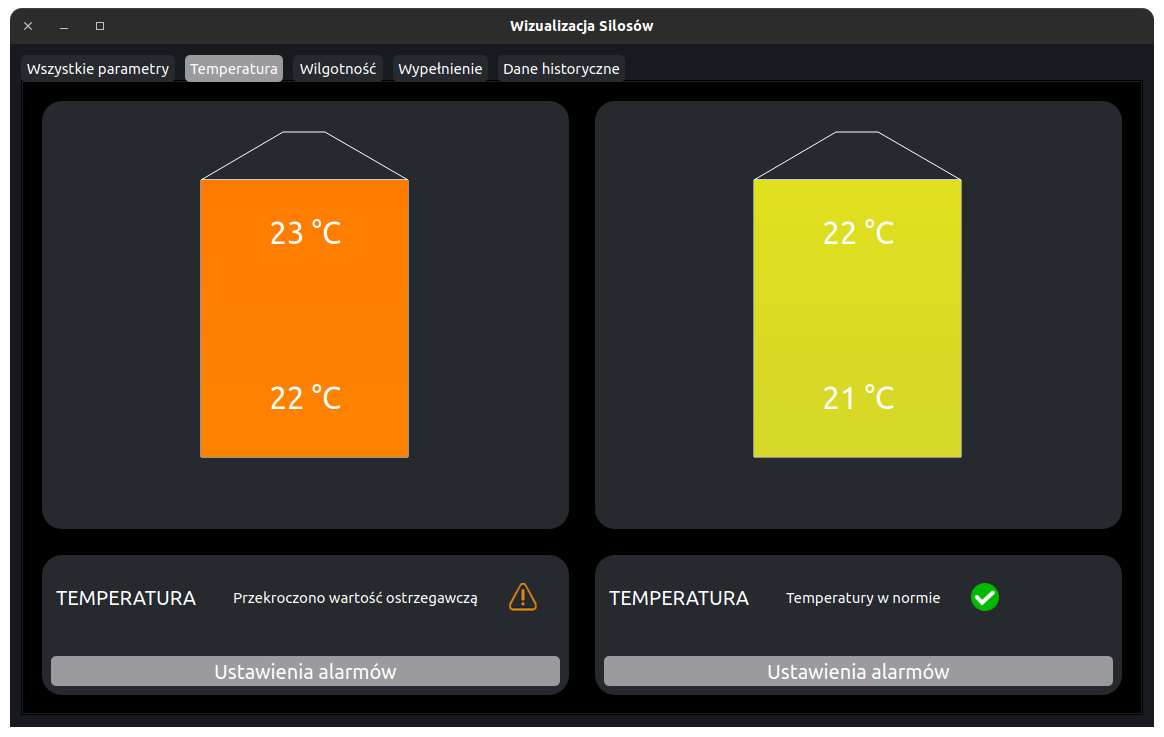
\includegraphics[width = \textwidth]{obrazy/temp_10_05.png}
                \caption{Wygląd zakładki Temperatura}
                \label{fig: temp 10 05}
            \end{figure}

            \begin{figure}[H]
                \centering
                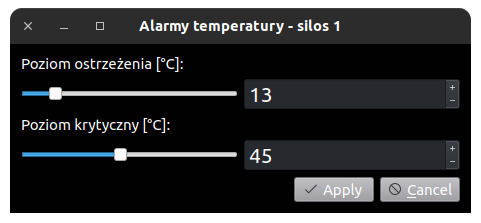
\includegraphics[width = \textwidth]{obrazy/alarm_window_10_05.png}
                \caption{Wygląd okienka pozwalającego na ustawienie wartości alarmów}
                \label{fig: alarms window 10 05}
            \end{figure}